\documentclass[12pt,letterpaper]{article}
\usepackage{graphicx,textcomp}
\usepackage{natbib}
\usepackage{setspace}
\usepackage{fullpage}
\usepackage{color}
\usepackage[reqno]{amsmath}
\usepackage{amsthm}
\usepackage{amssymb,enumerate}
\usepackage[all]{xy}
\usepackage{endnotes}
\usepackage{lscape}
\newtheorem{com}{Comment}
\newtheorem{lem} {Lemma}
\newtheorem{prop}{Proposition}
\newtheorem{thm}{Theorem}
\newtheorem{defn}{Definition}
\newtheorem{cor}{Corollary}
\newtheorem{obs}{Observation}
\usepackage[compact]{titlesec}
\usepackage{dcolumn}
\usepackage{tikz}
\usetikzlibrary{arrows}
\usepackage{multirow}
\usepackage{xcolor}
\newcolumntype{.}{D{.}{.}{-1}}
\newcolumntype{d}[1]{D{.}{.}{#1}}
\definecolor{light-gray}{gray}{0.65}
\usepackage{url}
\newcommand{\Sref}[1]{Section~\ref{#1}}
\newtheorem{hyp}{Hypothesis}

\title{Text as Data: Homework 1}
\date{}

\begin{document}
\maketitle

\subsubsection*{Question 1: Using Python}
\begin{itemize}
\item[a)] Install {\tt Python}, {\tt Rstudio}, and {\tt R markdown}
\item[b)] Using {\tt Python} write to a {\tt .txt} file:
\begin{itemize}
\item[-] {\tt Hello World}
\end{itemize}
With a for loop, write the numbers 1-100 to the same text file
\item[c)] Close the .txt file, turn it in with your homework
\end{itemize}




\subsubsection*{Question 2: Properties of Random Variables}  
\begin{itemize}
\item[a)] Suppose $X$ is a random variable, with $E[X] = \mu$ and var$(X) = \sigma^2$.  Show that $c = E[X]$ minimizes
\begin{eqnarray}
E[ (X - c)^2] \nonumber 
\end{eqnarray}
Why does this suggest $E[X]$ is a ``good" guess for the value of $X$?
\item[b)]  Suppose $Y$ and $Z$ are random variables, with joint density $f(y, z)$.  
\begin{itemize}
\item[i)] How do we obtain the marginal distribution of $Y$, $f_{Y}(y)$ (should be an expression involving an integral)
\item[ii)] How do we obtain the marginal distribution of $Z$, $f_{Z}(z)$ (should be an expression involving an integral)
\item[iii)] Show that if $Y$ and $Z$ are independent, $E[YZ] = E[Y]E[Z]$
\end{itemize} 
%\item[c)] \textbf{Iterated Expectations}: Suppose $Y$ and $Z$ are random variables, with joint density $f(y, z)$. Show that 
%\begin{eqnarray}
%E[Y] & = & E[ E[ Y|Z ] ] \nonumber \\
%& = & \int_{-\infty}^{\infty} \int_{-\infty}^{\infty} f_{Y|Z}(y|z)f_{Z}(z) dy dz \nonumber 
%\end{eqnarray}
\end{itemize}

\subsubsection*{Question 3: Finding Critical Values for a Function}

Suppose we have a function $f:\Re\rightarrow\Re$, $f(x) = \sin(x)$.  
\begin{itemize}
\item[a)] Using {\tt R} plot $\sin(x)$ for $x \in [-2 \pi, 2 \pi] $ (here $\pi$ is the mathematical constant). 
\item[b)] What is $f^{'}(x)$ (first derivative at $x$)?  Using {\tt R} plot it over $[-2 \pi, 2 \pi]$
\item[c)] What is $f^{''}(x)$ (second derivative at $x$)? Using {\tt R} plot it over $[-2 \pi, 2 \pi]$
\end{itemize}
We say that $x^{*}$ is a critical value for a function if $f^{'}(x^{*}) = 0$.  We can find $x^{*}$ algebraically. Or, we can use a computational approach.\\
\noindent We discussed the Newton-Raphson approach in class on Thursday.  We're going to write our own implementation of the algorithm in {\tt R} and apply it to find the critical values of $f(x) = \sin(x)$ 
\begin{itemize}
\item[d)] Suppose that we have current guess for the root $x_{t}$.  Then the updated guess, $x_{t+1}$ is given by
\begin{eqnarray}
x_{t+1} & = & x_{t} - \frac{f^{'}(x_{t})}{f^{''}(x_{t})} \nonumber 
\end{eqnarray}
\noindent where $f^{'}(x_{t})$ is the first derivative evaluated at $x_{t}$ and $f^{''}(x_{t})$ is the second derivative evaluated at $x_{t}$.  \\
\noindent Write a function in {\tt R} that provides the update step for some value $x_{t}$ if $f(x) = \sin(x)$.  
\item[e)] The Newton-Raphson algorithm continues to update until the size of the update step drops below a threshold.  Using the {\tt while} command in R, write a loop that continues updating until the change,( $|x_{t+1} - x_{t}|$) drops below $10^{-5}$.  
\item[f)] Place the while loop in a function that returns the converged value $x_{\text{final}}$
\item[g)] Use your function with initial guesses $-2, -1, 1, 2$.  What values do you obtain?  Now examine the behavior close to $0$.  Why is it so unstable?
\end{itemize}

\begin{table}[hbt!]
\caption{Pseudo Code for Newton Raphson (To assist in developing your function)}
\begin{itemize}
\item $x_{0}$ = initial guess
\item Do while change $>$ tolerance:
\begin{itemize}
\item[] $x_{t+1}  = x_{t} - \frac{f^{'}(x_{t})}{f^{''}(x_{t} ) } $
\item[] change = $| x_{t+1} - x_{t}|$ 
\end{itemize}
\item return $x_{t+1}$
\end{itemize}
\end{table}


\subsubsection*{Problem 3: Probit Regression with a Prior}

Suppose that we assume the following data generation process
\begin{eqnarray}
Y_{i} & \sim & \text{Bernoulli}(\pi_{i} ) \nonumber \\
\pi_{i} & = & \Phi(\boldsymbol{X}_{i} \boldsymbol{\beta}) \nonumber \\
\beta_{j} & \sim & \text{Normal}(\mu, \sigma^{2}_{j} )\nonumber 
\end{eqnarray}

with $\boldsymbol{X}_{i} = (1, x_{i})$ for all $i$ $(i = 1, \hdots, N)$,  $\boldsymbol{\beta} = (\beta_{1}, \beta_{2})$, and $\Phi(\cdot)$ is the cumulative normal distribution function.  \\

We might equivalently write a directed acyclic graph as, 

\vspace{0.25in}

\begin{large}
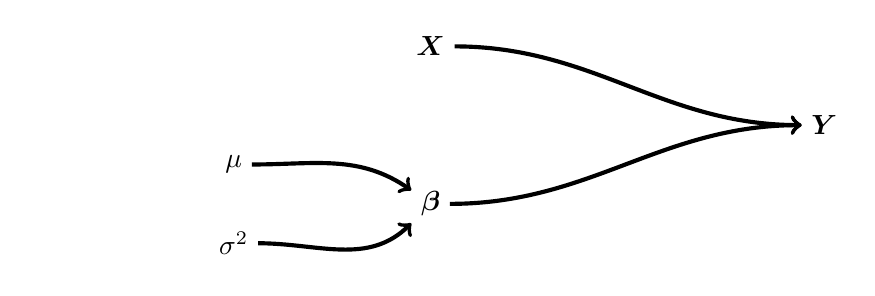
\begin{tikzpicture}
\node(dummy) at (-8, 8) [] {} ; 
\node(covariates) at (-3, 9) [] {$\boldsymbol{X}$} ; 
\node(betas) at (-3, 7) [] {$\boldsymbol{\beta}$ } ; 
\node(prior1) at (-5.5, 7.5) [] {$\mu$ } ; 
\node(prior2) at (-5.5, 6.5) [] {$\sigma^2$ } ; 
\node(dependent) at (2, 8) [] {$\boldsymbol{Y}$};
\draw[->, line width = 1.5pt] (prior1) to [out = 0, in = 145] (betas) ; 
\draw[->, line width = 1.5pt] (prior2) to [out = 0, in = 225] (betas) ; 
\draw[->, line width = 1.5pt] (covariates) to [out = 0, in= 180] (dependent) ; 
\draw[->, line width = 1.5pt] (betas) to [out = 0, in= 180] (dependent) ; 
\end{tikzpicture}
\end{large}


This is very similar to the model described in class, but now we have added a \emph{prior} on $\boldsymbol{\beta}$.  This slightly alters the objective function:

\begin{eqnarray}
p(\boldsymbol{\beta} | \boldsymbol{Y}, \boldsymbol{X}) & \propto & p(\boldsymbol{\beta}|\mu, \sigma^2) \times p(\boldsymbol{Y}| \boldsymbol{X}, \boldsymbol{\beta}) \label{e:post} \\
& \propto &  \prod_{j=1}^{2} \frac{1}{\sqrt{2\pi} \sigma} \exp\left( - \frac{(\beta_{j} - \mu)^2}{2 \sigma^2} \right) \times \prod_{i=1}^{N} \Phi(\boldsymbol{X}_{i}\boldsymbol{\beta})^{Y_{i} } ( 1- \Phi(\boldsymbol{X}_{i}\boldsymbol{\beta})^{1 - Y_{i} } \nonumber 
\end{eqnarray}

In this problem, we will examine how the prior on $\boldsymbol{\beta}$, and in particular the values we set for $\mu$ and $\sigma^2$, alters our inferences about $\boldsymbol{\beta}$.

\begin{itemize}
\item[a)] Analytically, write out the $\log(p(\boldsymbol{\beta} | \boldsymbol{Y}, \boldsymbol{X}))$.  
\item[b)] In {\tt R} create a function for the $\log$ of Equation \ref{e:post}.
\item[c)] Using the synthetic data and the optim guide from class, use {\tt optim} to find $\widehat{\boldsymbol{\beta}}$ with $\mu = 0$ and $\sigma^2 = 1000$
\item[d)] Set $\mu = 1$ and then vary $\sigma^2$.  Using a {\tt for} loop, store estimates of how $\beta_{2}$ changes as you vary $\sigma^2$ from $10$ to $0.01$.  Plot $\beta_{2}$ against $\sigma^2$ and describe what happens as $\sigma^2$ varies.  
\end{itemize}


\end{document}